\section{An\'alisis de estabilidad}

Para simular la ganancia de lazo de cada celda, se pasiv\'o la entrada al circuito, se puso una fuente en la entrada de un op-amp tal como se muestra en la figura \ref{fig:loop_gain_sim}, y se obtuvo el cociente entre el borne negativo y el positivo de la fuente. Una vez obtenida esta transferencia, se calcula el margen de fase y de ganancia de cada celda (tabla \ref{tab:margenes_estabilidad}).

\begin{figure}[H]
	\centering
	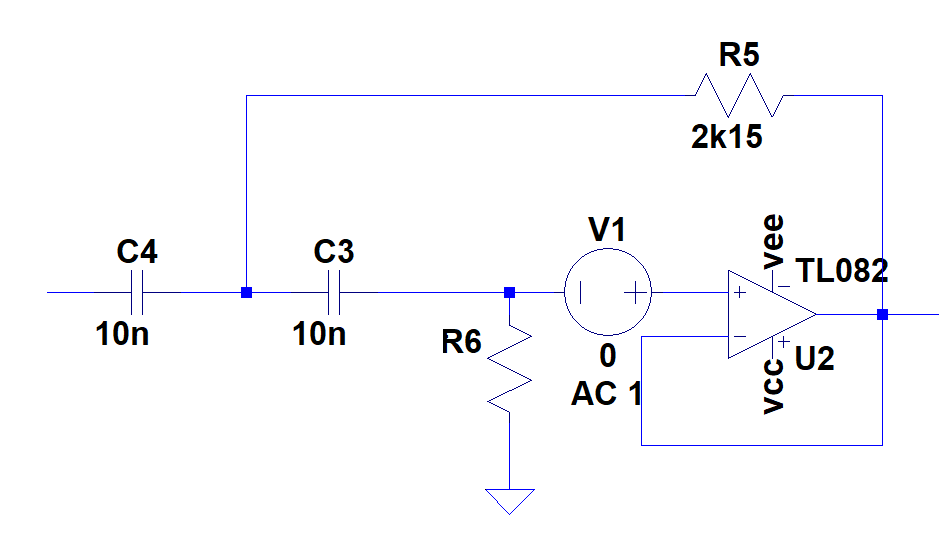
\includegraphics[scale=0.5]{imagenes/loop_gain_sim}
	\caption{Simulaci\'on de ganancia de lazo de la segunda celda (Sallen-Key pasaaltos) en LTspice}
	\label{fig:loop_gain_sim}
\end{figure}

\begin{table}[H]
	\centering
	\begin{tabular}{||c c c||}
	\hline 
	Etapa & Margen de fase & Margen de ganancia \\ 
	\hline 
	\hline
	1 & --- & 60dB \\ 
	
	2 & --- & 2dB \\ 
	
	3 & --- & 3dB \\ 
	
	4 & 10$^\circ$ &  25dB\\ 
	
	5 & 10$^\circ$ & 15dB \\ 
	\hline
	\end{tabular} 
	\label{tab:margenes_estabilidad}
\end{table}

Los m\'argenes de fase y de ganancia no son grandes. Por este motivo se buscaron oscilaciones en el circuito y no se hallaron.

\begin{figure}[H]
	\centering
	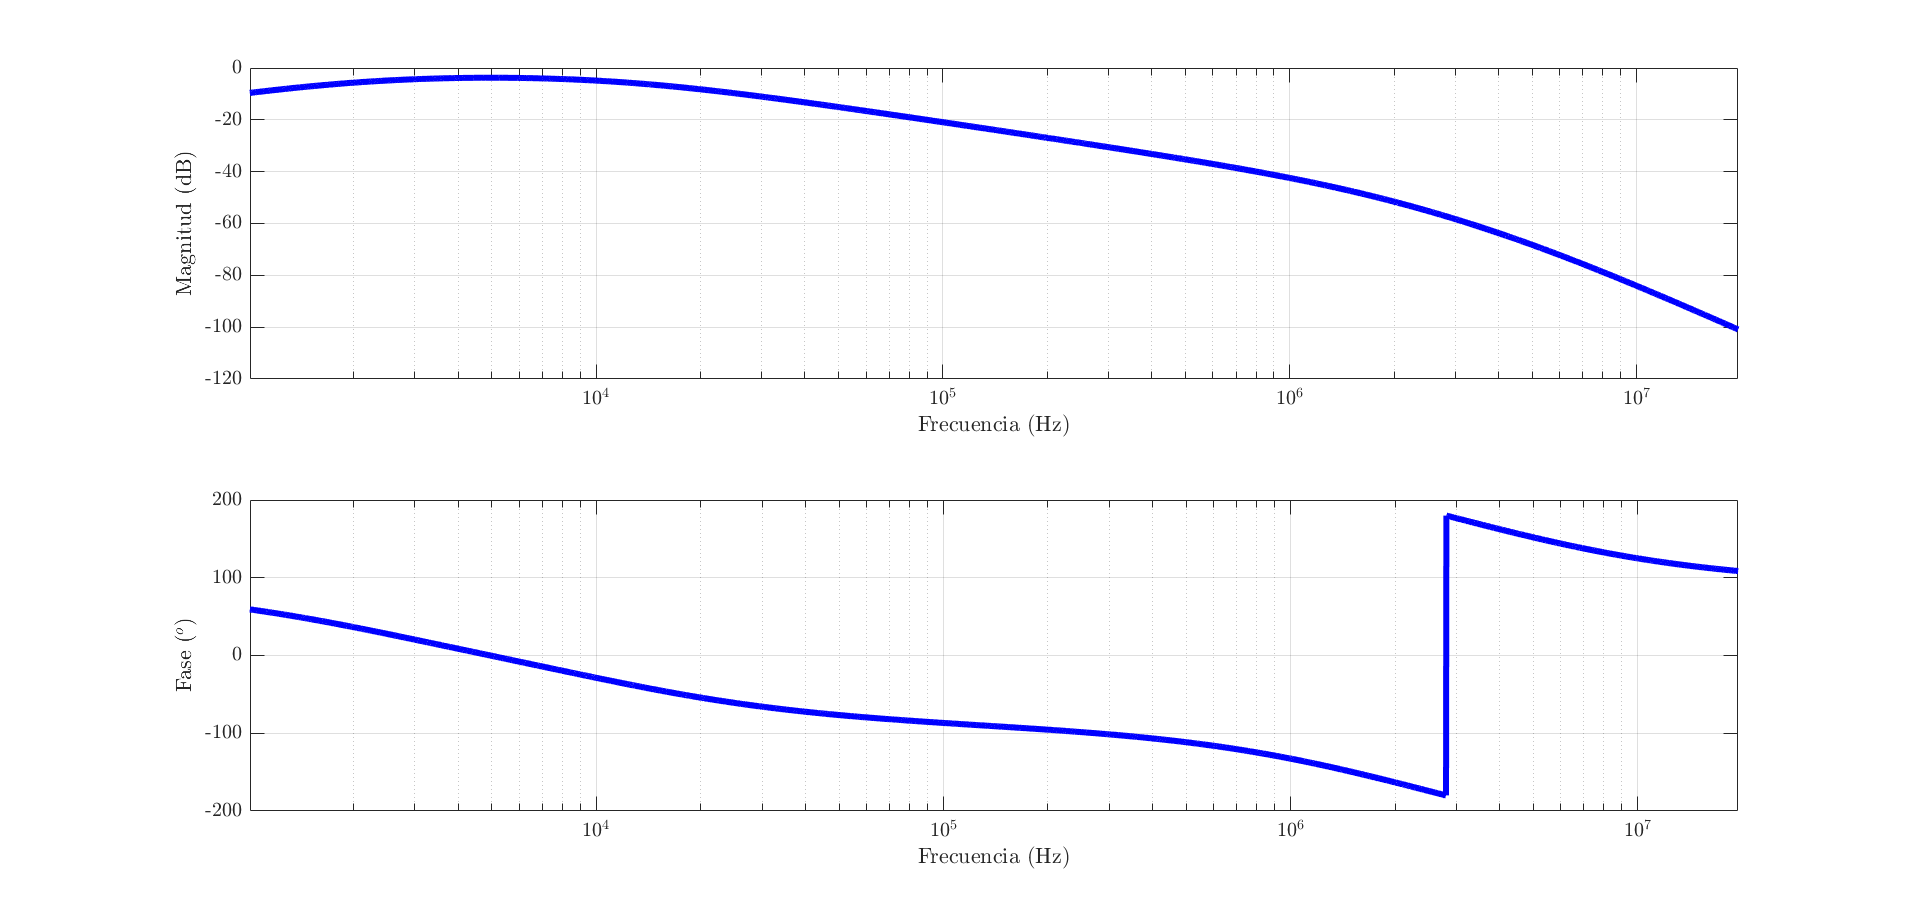
\includegraphics[width = \textwidth]{imagenes/estabilidad_etapa_1_v1}
	\caption{Ganancia de lazo de la primer etapa (Sallen-Key pasabanda)}
	\label{fig:loop_gain_1}
\end{figure}
\begin{figure}[H]
	\centering
	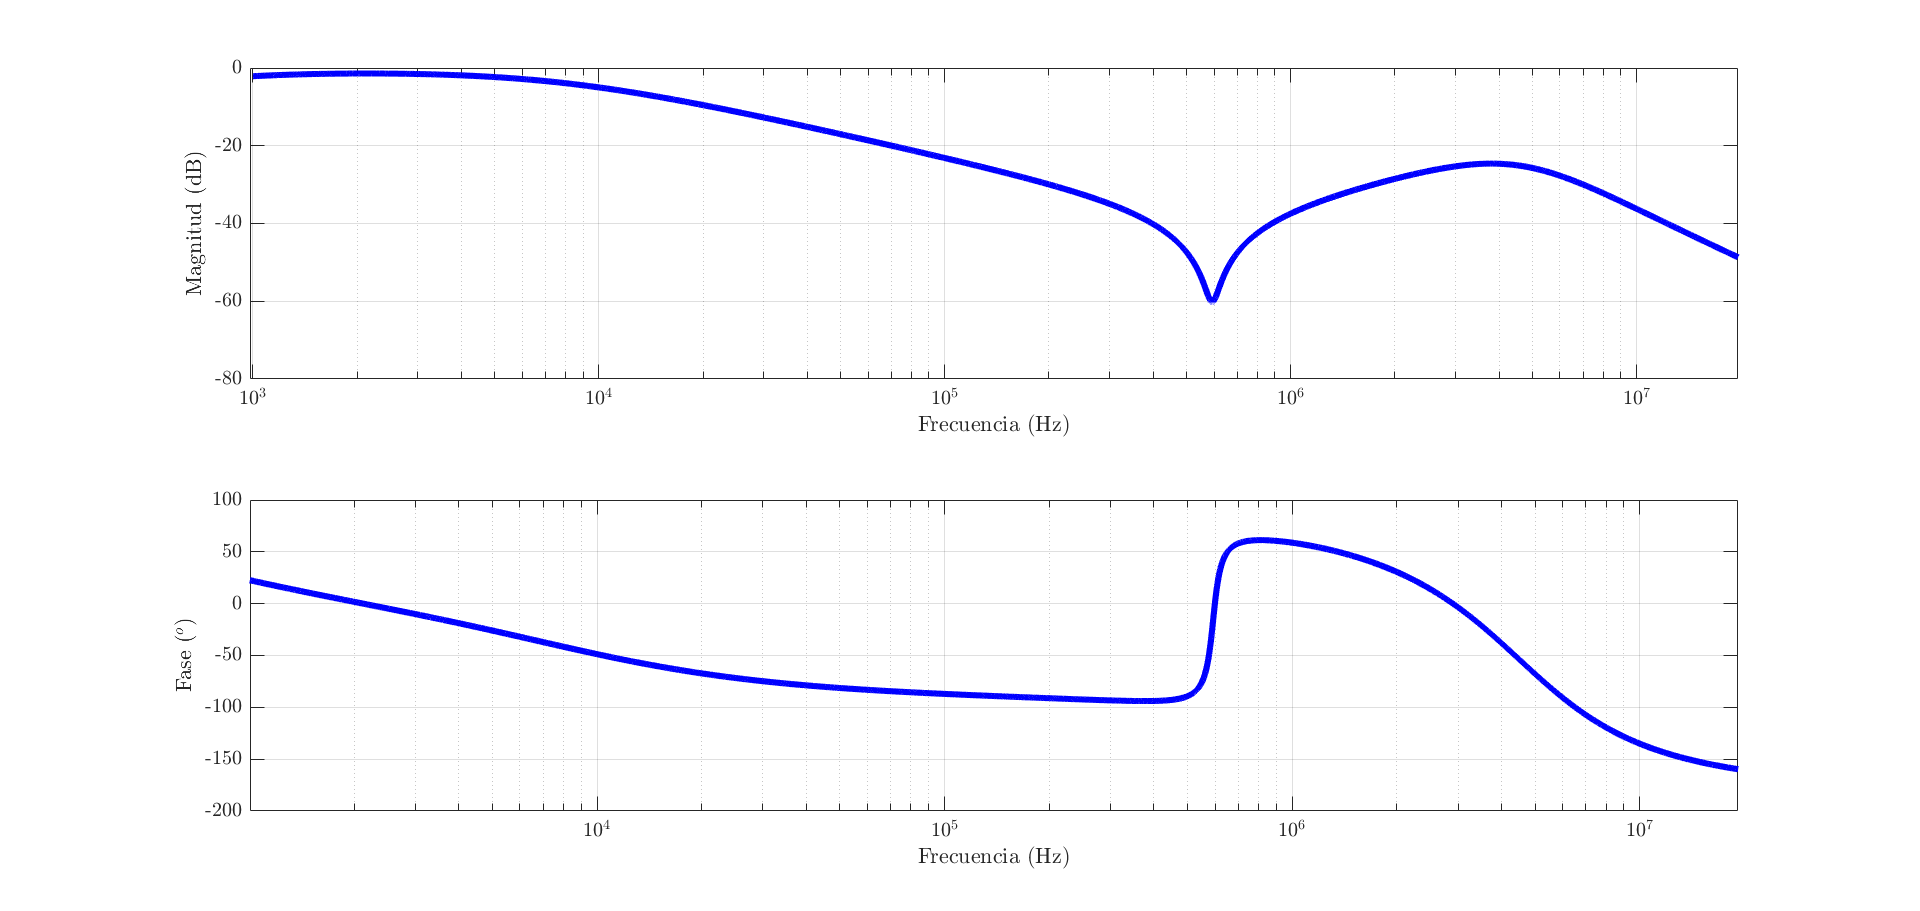
\includegraphics[width = \textwidth]{imagenes/estabilidad_etapa_2_v1}
	\caption{Ganancia de lazo de la segunda etapa (Sallen-Key pasaaltos)}
	\label{fig:loop_gain_2}
\end{figure}
\begin{figure}[H]
	\centering
	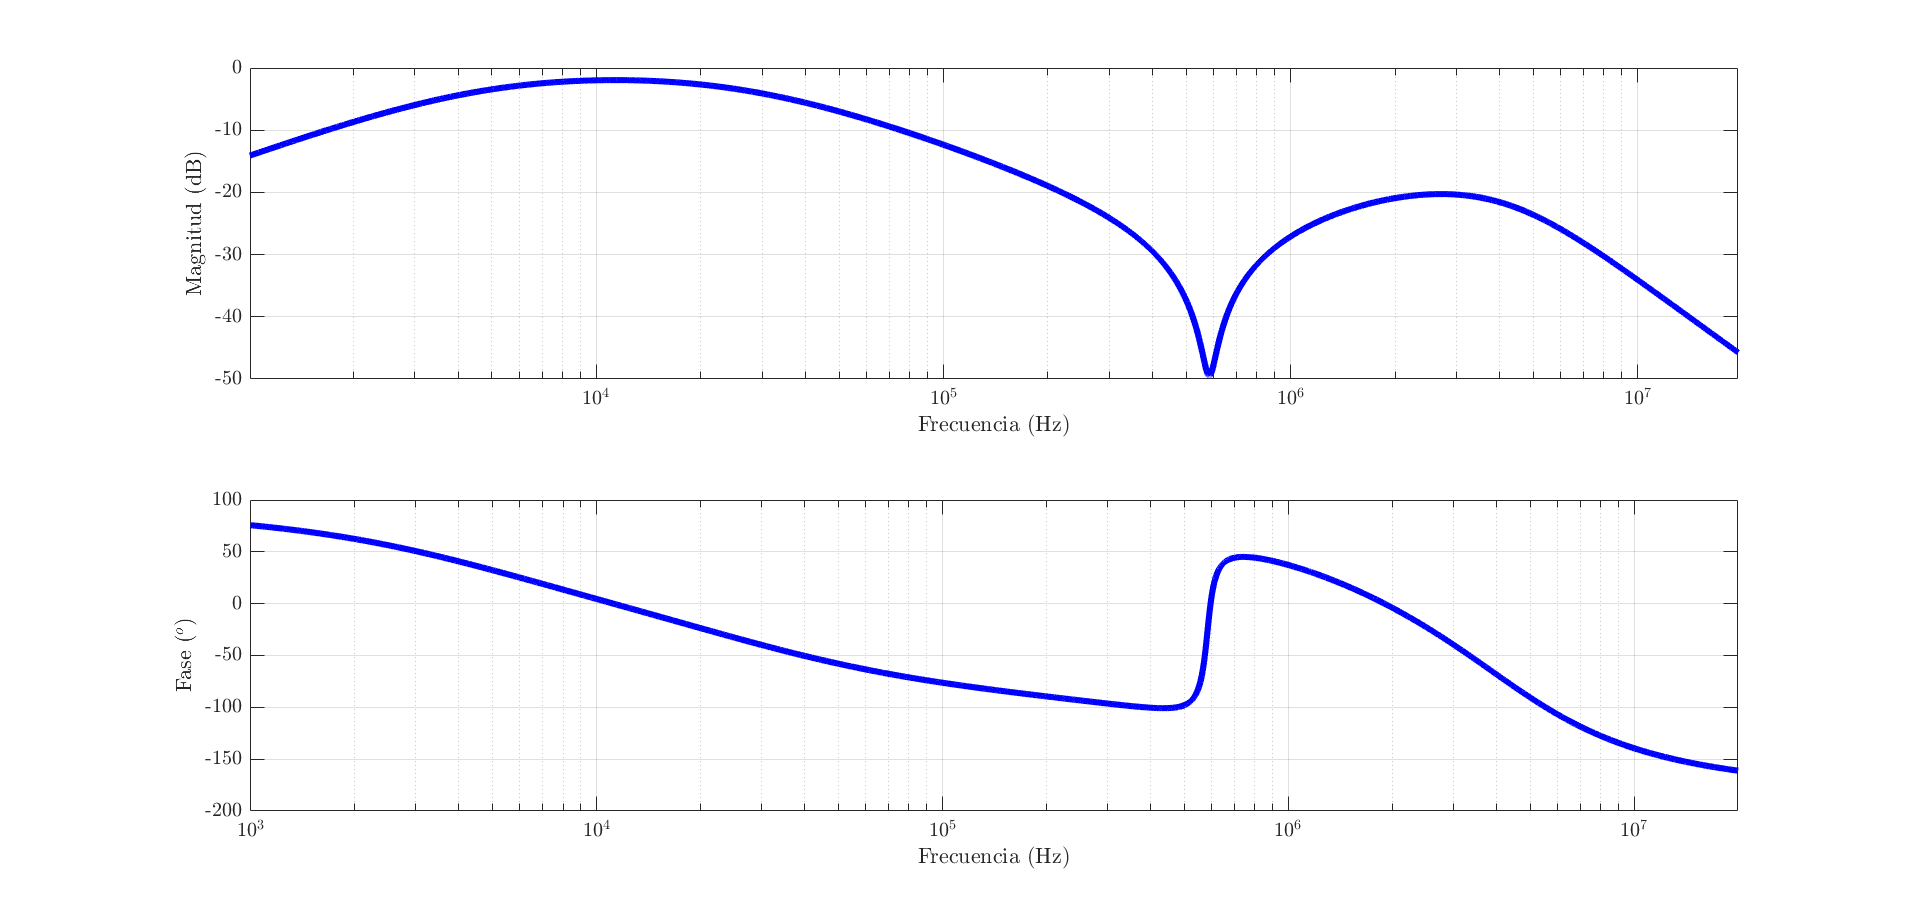
\includegraphics[width = \textwidth]{imagenes/estabilidad_etapa_3_v1}
	\caption{Ganancia de lazo de la tercer etapa (Sallen-Key pasaaltos)}
	\label{fig:loop_gain_3}
\end{figure}
\begin{figure}[H]
	\centering
	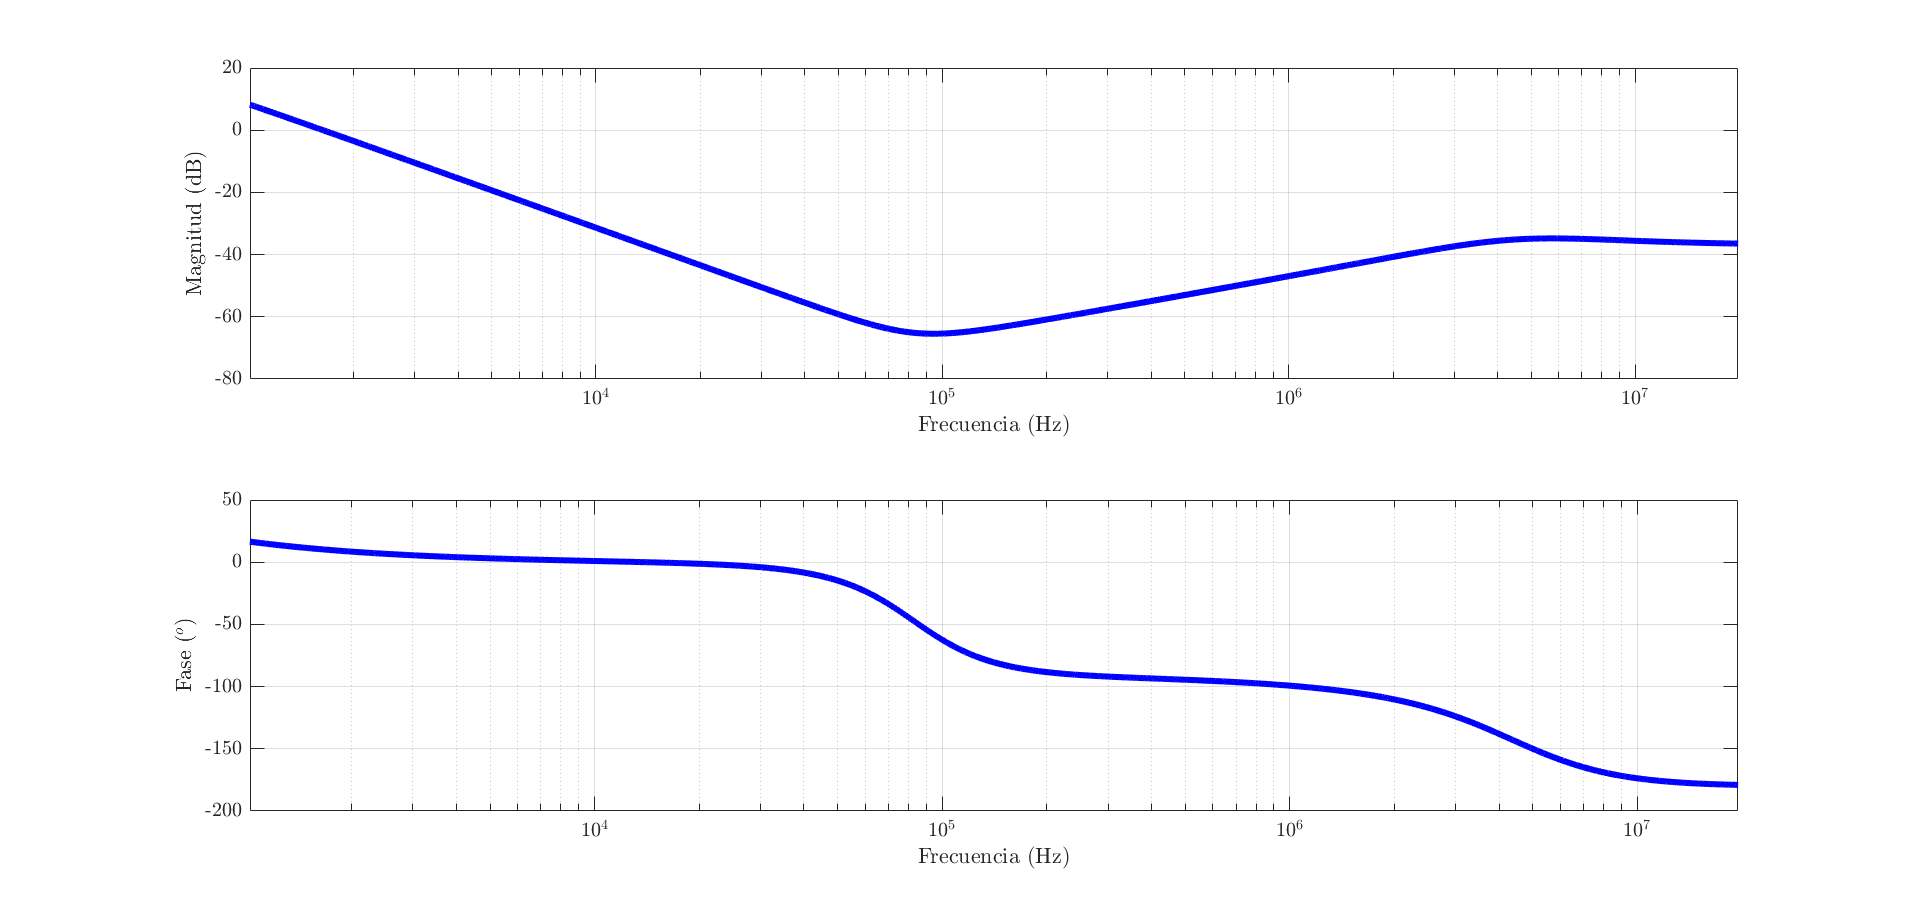
\includegraphics[width = \textwidth]{imagenes/estabilidad_etapa_4_v1}
	\caption{Ganancia de lazo de la cuarta etapa (Tow-Thomas pasabajos)}
	\label{fig:loop_gain_4}
\end{figure}
\begin{figure}[H]
	\centering
	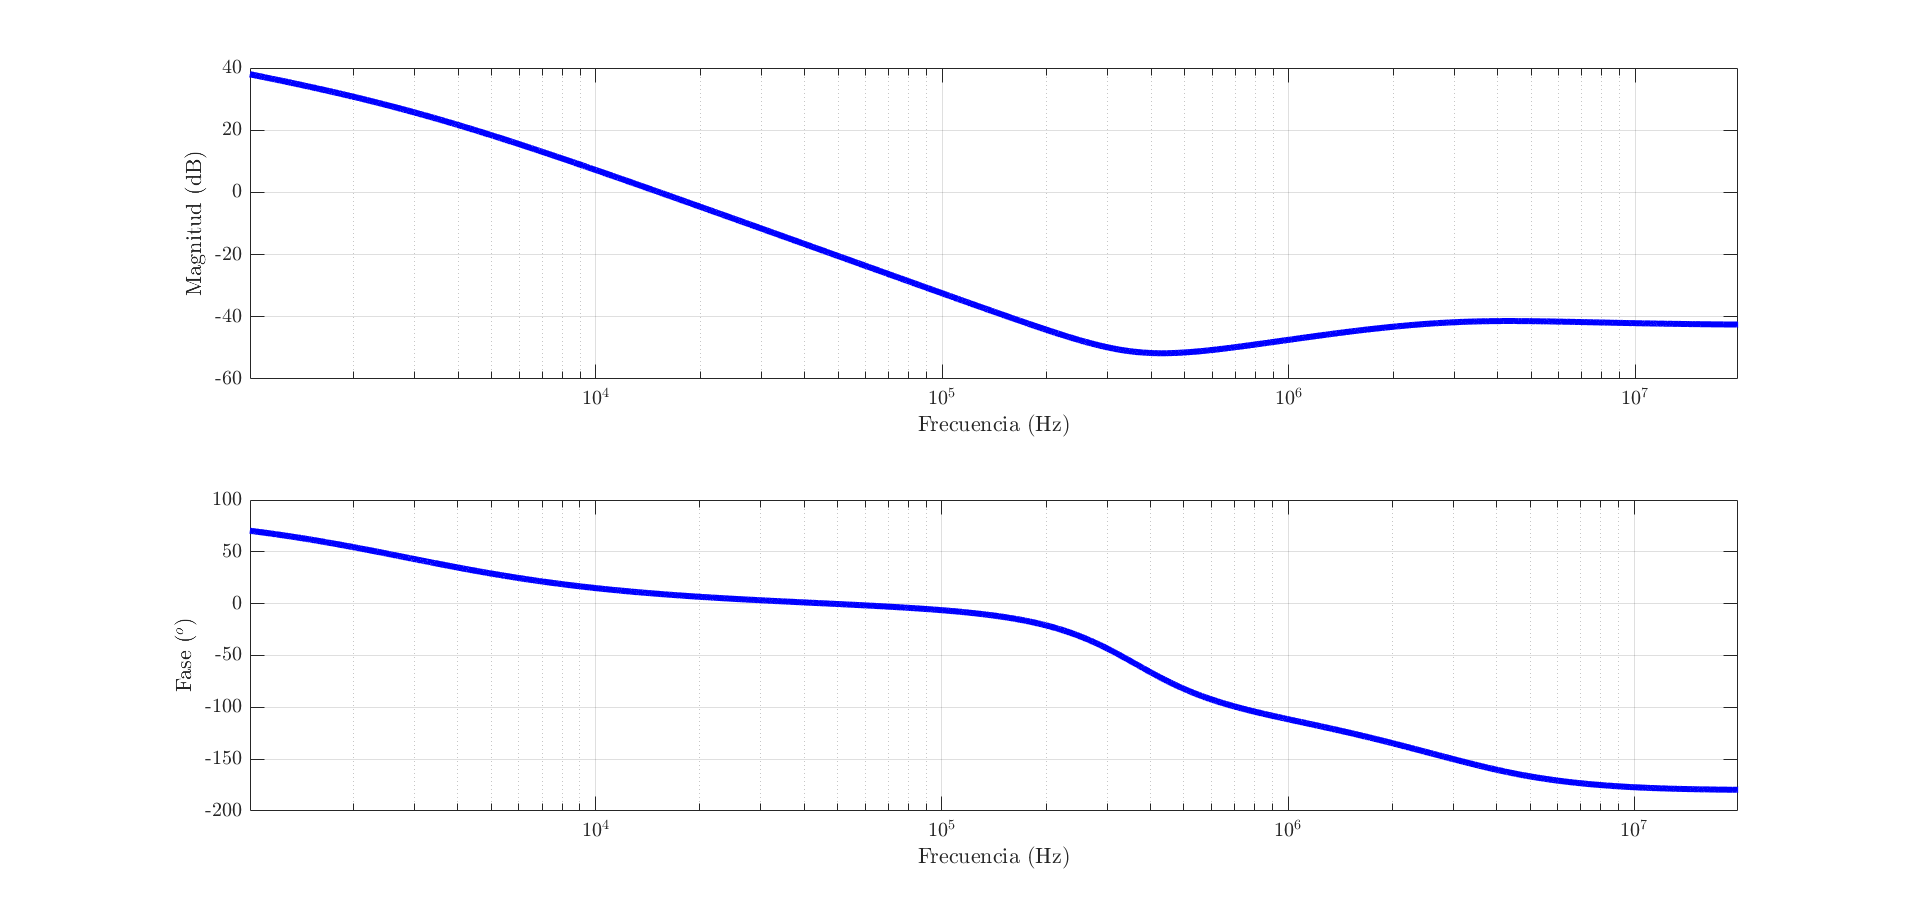
\includegraphics[width = \textwidth]{imagenes/estabilidad_etapa_5_v1}
	\caption{Ganancia de lazo de la quinta etapa (Tow-Thomas pasabajos)}
	\label{fig:loop_gain_5}
\end{figure}
